% -*- coding=utf-8 -*-
\chapter{写作示例}
\section{列表环境}

\subsection{无序列表}

使用环境\verb+itemize+是一个无序列表的例子,列表的每个条目单独分段。

\begin{itemize}
	\item 这是一个无序列表。
	\item 这是一个无序列表。
	\item 这是一个无序列表。
\end{itemize}

\subsection{有序列表}

使用环境\verb+enumerate+创建有序列表,使用方法与无序列表类似。

\begin{enumerate}[label={\arabic*}]
	\item 这是一个有序列表。
	\item 这是一个有序列表。
	\item 这是一个有序列表。
\end{enumerate}

通过修改\verb+enumerate+环境后的参数\verb+[label={\arabic*}]+可以实现编号数字类型的切换。
\verb+\arabic+可以替换为\verb+\roman+,\verb+\Roman+,\verb+\alph+,\verb+\Alph+来表示小写罗马数字,大写罗马数字,小写字母编号,大写字母编号。

可以加入一些括号让列表更加好看,例如:\verb+[label={\roman*)}]+显示效果如下

\begin{enumerate}[label={\roman*)}]
	\item 这是一个有序列表。
	\item 这是一个有序列表。
	\item 这是一个有序列表。
\end{enumerate}
\subsection{描述列表}
使用环境\verb+description+可创建带有主题词的列表,条目语法是\verb+\item[主题] 内容+。示例如下:

\begin{description}
	\item[主题一] 详细内容
	\item[主题二] 详细内容
	\item[主题三] 详细内容 \ldots
\end{description}

\section{数学排版}

\subsection{公式排版}

这里有举一个长公式排版的例子,来自\href{http://www.tex.ac.uk/tex-archive/info/math/voss/mathmode/Mathmode.pdf}{《Math mode》}:
\begin{multline}
\frac {1}{2}\Delta (f_{ij}f^{ij})=
2\left (\sum _{i<j}\chi _{ij}(\sigma _{i}-
\sigma _{j}) ^{2}+ f^{ij}\nabla _{j}\nabla _{i}(\Delta f)+\right .\\
\left .+\nabla _{k}f_{ij}\nabla ^{k}f^{ij}+
f^{ij}f^{k}\left [2\nabla _{i}R_{jk}-
\nabla _{k}R_{ij}\right ]\vphantom {\sum _{i<j}}\right )
\end{multline}

\subsection{定理环境}

在这个模板中,我们有如下几个环境:definition(定义),theorem(定理),lemma(引理),corollary(推论),remark(注),example(例)。
amsmath还提供了一个proof(证明)的环境。

其中,定义,定理,引理按section连续编号,推论,注,例按chapter单独编号。
我们举例说明它们的用法。

定义环境
\begin{definition}[域]\label{def:field}
	设$S$为一个非空集合,其上有“加法”(记作$+$)与“乘法”(记作$\cdot$)两种代数运算. 若满足以下条件,则称$(S,+,\cdot)$构成一个域(field).
	\begin{enumerate}[label={\rm{\roman*)}}]
		\item $(S,+)$构成一个交换群.
		\item 若记$S^{*}=S-\{0\}$,其中$0$为群$(S,+)$中的单位元,则$(S^{*},\cdot)$也构成一个交换群.
		\item 乘法对加法有分配律:$a ( b + c ) = a b + a c$.
	\end{enumerate}
\end{definition}

引理环境
\begin{lemma}\rm{\cite{Azizov2003On}}\label{lem:Weierstrass}
	实轴上任一有界无限点集$S$至少有一个聚点。
\end{lemma}

推论环境
\begin{corollary}
	根据引理\ref{lem:Weierstrass},我们可以得到柯西收敛准则。
\end{corollary}

定理环境
\begin{theorem}[望远镜公式]\label{thm:telescope}
	$\left[\mathbb{Q}(a, b) : \mathbb{Q}\right]=\left[\mathbb{Q}(a, b) : \mathbb{Q}(a)\right]\left[\mathbb{Q}(a) : \mathbb{Q}\right] $
\end{theorem}

注环境
\begin{remark}\label{rem:reversible}
	每个操作都可逆。
\end{remark}

证明环境
\begin{proof}
	\autoref{thm:telescope} 告诉我们,对任意$s\in S$,均有$\lvert Orb(s)\rvert \cdot \lvert Stab(s)\rvert=\lvert G\rvert=p$。 于是$\lvert Orb(s)\rvert $整除$p$,这里$p$是一个素数。
	从而$\lvert Orb(s)\rvert $等于1或$p$,也就是说,\textbf{所有轨道的大小要么为1,要么为$p$}。
	于是整个集合$S$就被划分为两部分,一部分是大小为1的轨道,另一部分是大小为$p$的轨道,如图9.4所示。
	
	假设大小为1的轨道有$m$个,大小为$p$的轨道有$n$个,则有
	\begin{equation}
		m+p\cdot n=\lvert S\rvert 
	\end{equation}
	注意到定义\ref{def:field},\textbf{那些$\lvert Orb(s)\rvert =1$的元素$s$即为稳定元},这就表明有$m$个稳定元。从上式立刻看出$\lvert S \rvert \equiv  m\; (\bmod\; p)$。
\end{proof}
 

例子环境
\begin{example}
	用数列的柯西准则证明确界有界。
\end{example}

\section{表格}
学术论文的表格一般采用三线表格式,这里提供两个模板,一个是简单的模板,另一个个支持表格跨页。

{
\songti\zihao{5}  % 五号宋体,没找到合适的全局设置
\begin{table}[htbp]
  \centering
  \caption{普通表格}
  \label{tab:pinci}
    \begin{tabularx}{0.9\textwidth} { 
        >{\centering\arraybackslash}X 
        >{\centering\arraybackslash}X 
        >{\centering\arraybackslash}X 
        >{\centering\arraybackslash}X 
        }
        \toprule
        表头 & 表头 & 表头 & 表头 \\
        \midrule
        内容 & 内容 & 内容 & 内容 \\
        内容 & 内容 & 内容 & 内容 \\
        内容 & 内容 & 内容 & 内容 \\
        内容 & 内容 & 内容 & 内容 \\
        \bottomrule
    \end{tabularx}
\end{table}
}

{
\songti\zihao{5}
\begin{longtable}{%
    >{\centering\arraybackslash}m{0.2\textwidth} % 25% of text width for the first column
    >{\centering\arraybackslash}m{0.2\textwidth} % 25% of text width for the second column
    >{\centering\arraybackslash}m{0.2\textwidth} % 25% of text width for the third column
    >{\centering\arraybackslash}m{0.2\textwidth} % 25% of text width for the fourth column
}
  \caption{支持跨页的表}
  \label{tab:guanlian} \\
  \toprule
  表头 & 表头 & 表头 & 表头 \\
  \midrule
  \endfirsthead
  \multicolumn{4}{c}{{\tablename\ \thetable{} 续表}} \\
  \toprule
  后项 & 前项 & 支持度百分比 & 置信度百分比 \\
  \midrule
  \endhead
  \bottomrule
  \multicolumn{4}{r}{{转下页}}
  \endfoot
  \bottomrule
  \endlastfoot

  % 表格内容...
  内容 & 内容 & 内容 & 内容 \\
  内容 & 内容 & 内容 & 内容 \\
  内容 & 内容 & 内容 & 内容 \\
  内容 & 内容 & 内容 & 内容 \\
  内容 & 内容 & 内容 & 内容 \\
  内容 & 内容 & 内容 & 内容 \\
  内容 & 内容 & 内容 & 内容 \\
  内容 & 内容 & 内容 & 内容 \\
  内容 & 内容 & 内容 & 内容 \\
  内容 & 内容 & 内容 & 内容 \\
  内容 & 内容 & 内容 & 内容 \\
  内容 & 内容 & 内容 & 内容 \\
  内容 & 内容 & 内容 & 内容 \\
  内容 & 内容 & 内容 & 内容 \\
  内容 & 内容 & 内容 & 内容 \\
  内容 & 内容 & 内容 & 内容 \\
  内容 & 内容 & 内容 & 内容 \\
  内容 & 内容 & 内容 & 内容 \\
  内容 & 内容 & 内容 & 内容 \\
  内容 & 内容 & 内容 & 内容 \\
  内容 & 内容 & 内容 & 内容 \\
  内容 & 内容 & 内容 & 内容 \\
  内容 & 内容 & 内容 & 内容 \\
  内容 & 内容 & 内容 & 内容 \\
  内容 & 内容 & 内容 & 内容 \\
  内容 & 内容 & 内容 & 内容 \\
  内容 & 内容 & 内容 & 内容 \\
  内容 & 内容 & 内容 & 内容 \\
  内容 & 内容 & 内容 & 内容 \\
  内容 & 内容 & 内容 & 内容 \\
  内容 & 内容 & 内容 & 内容 \\
  内容 & 内容 & 内容 & 内容 \\
  内容 & 内容 & 内容 & 内容 \\
  内容 & 内容 & 内容 & 内容 \\
\end{longtable}
}

\section{插入图片}

XeLatex 可以很方便地插入PDF、PNG、JPG格式的图片。插入PNG/JPG的例子如\autoref{fig1}所示。
这两个水平并列放置的图共享一个“图标题”(table caption),没有各自的小标题。

\begin{figure}[htp]
	\centering
	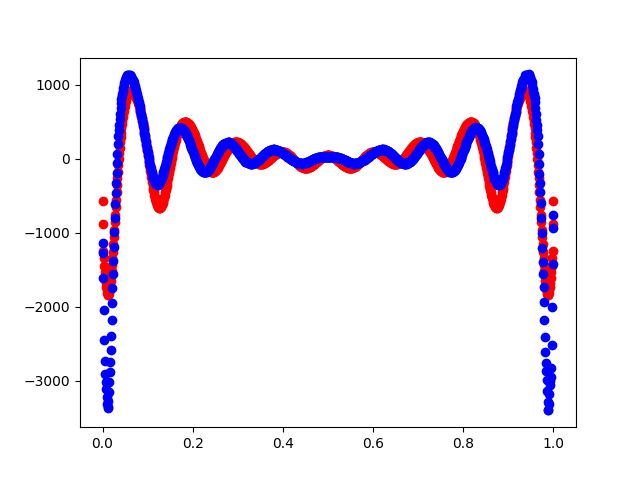
\includegraphics[width=6cm]{figure/example/model1_1000.png}
	\hspace{1cm}
	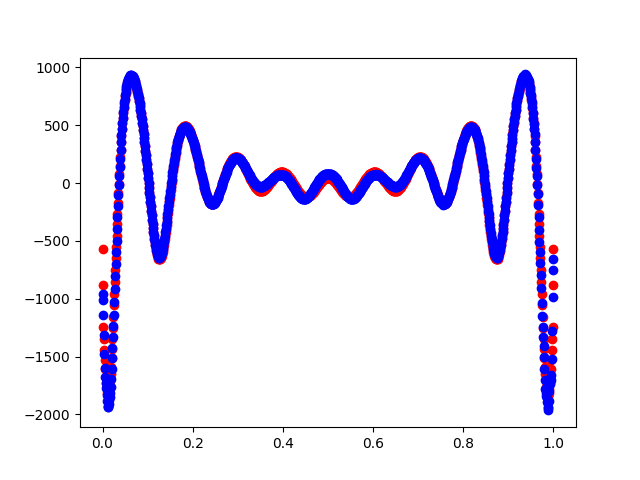
\includegraphics[width=6cm]{figure/example/model1_10000.png}
	\bicaption{中文题图}
	{English caption}
	\label{fig1}
\end{figure}

这里还有插入EPS图像和PDF图像的例子,如\autoref{fig2} 和\autoref{fig3}。这里将EPS和PDF图片作为子图插入,每个子图有自己的小标题。子图标题使用subcaption宏包添加。

\begin{figure}[htp]
	\centering
	\subcaptionbox{PDF 图像\label{fig2}}[3cm] %标题的长度,超过则会换行,如下一个小图。
	{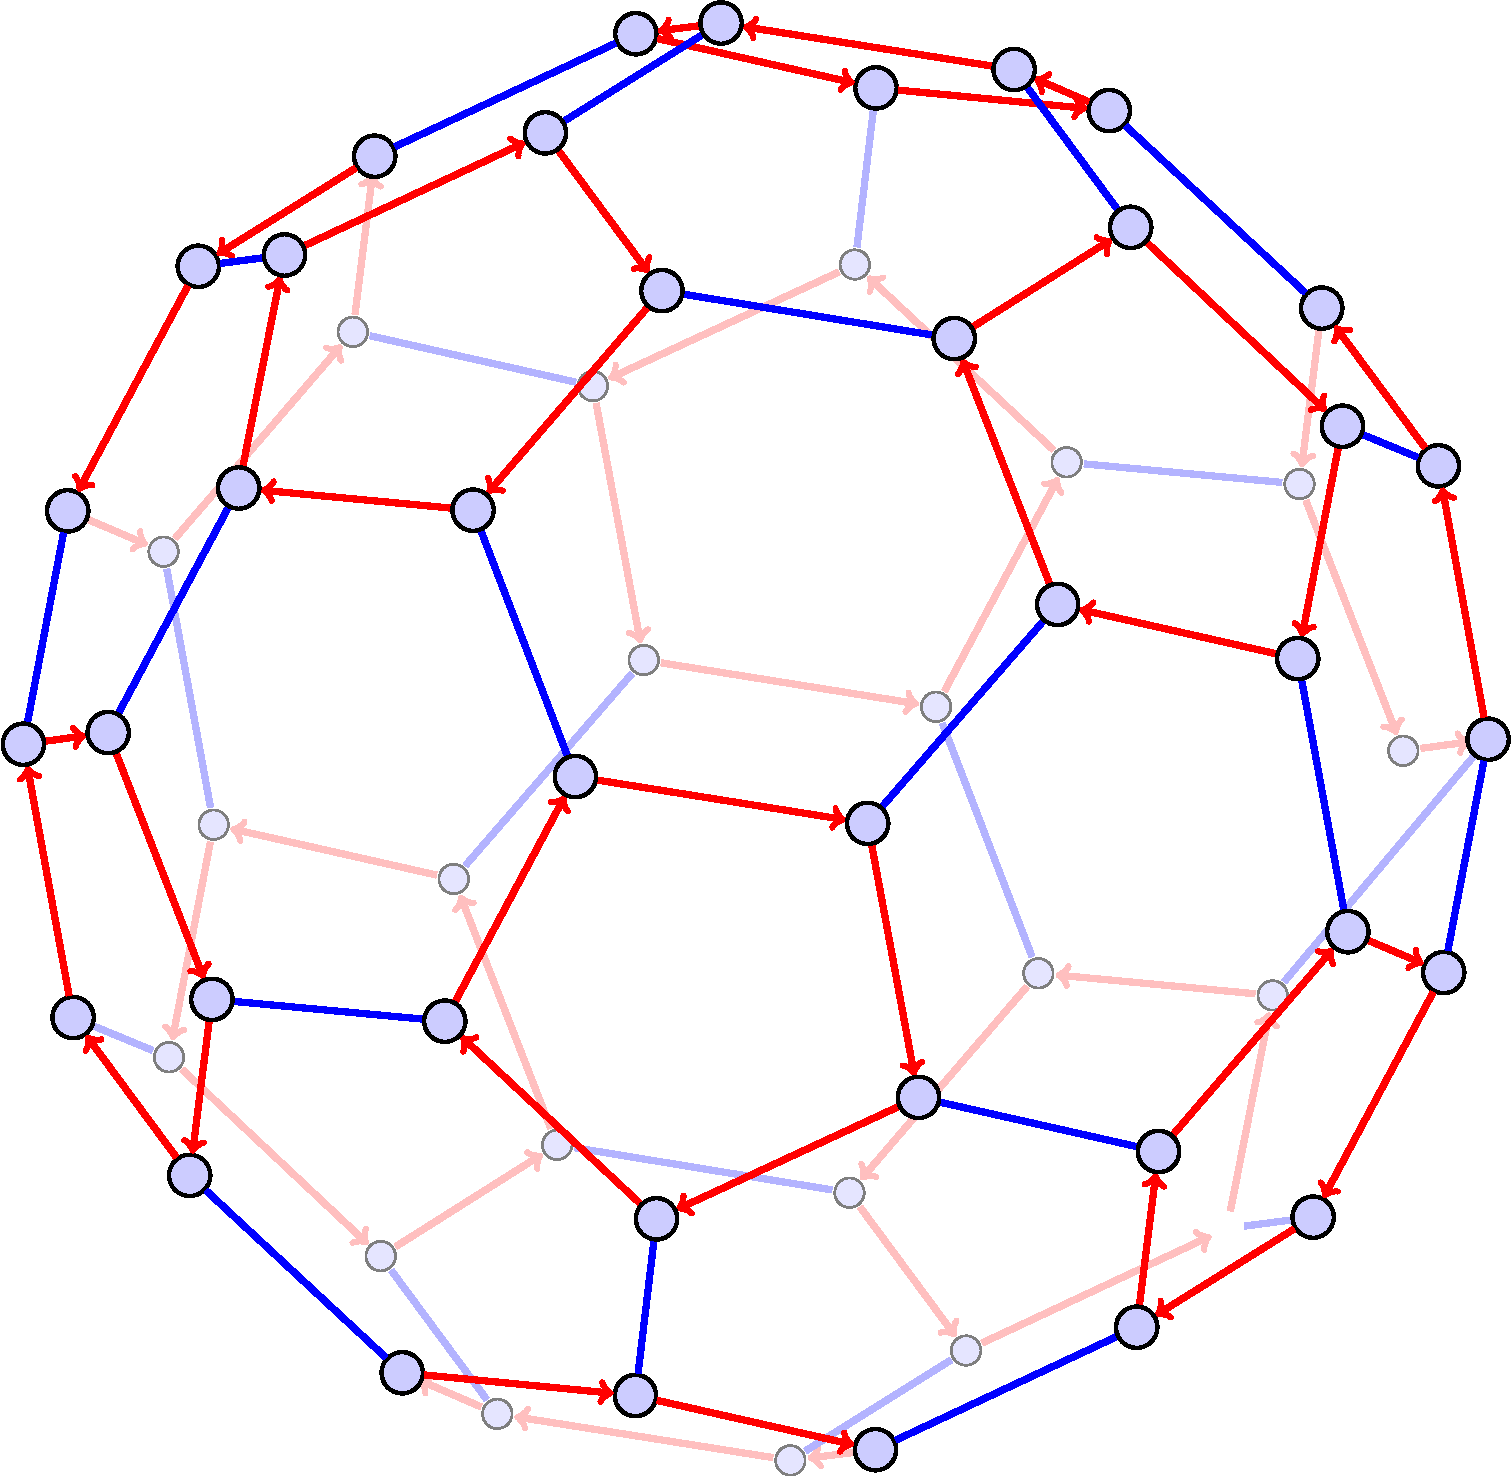
\includegraphics[height=2.5cm]{figure/example/m2.pdf}}
	\hspace{4em}
	\subcaptionbox{EPS 图像,如果标题很长的话,它会自动换行\label{fig3}}
	{	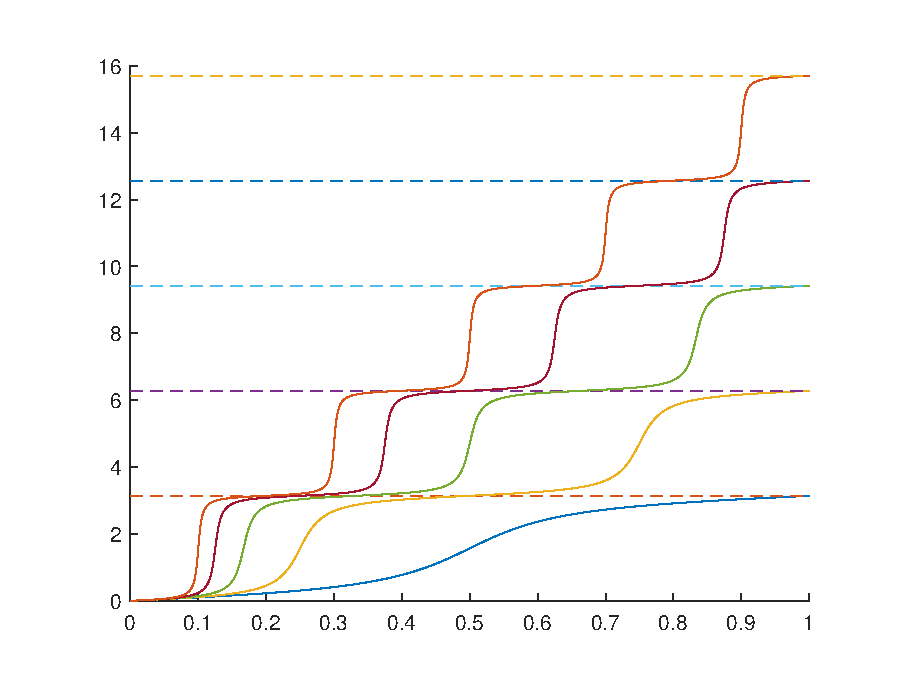
\includegraphics[scale=0.5]{figure/example/purfer_left.eps}}
	\bicaption{插入eps和pdf的例子(使用 subcaptionbox 方式)}{An EPS and PDF demo with subcaptionbox}
	\label{fig4}
\end{figure}。

\section{插入代码}

这里给一个使用listings宏包插入源代码的例子:
\begin{lstlisting}[language={C}, caption={一段C源代码}, label=code:1]
#include <stdio.h>

int main() {
    printf("Hello World!\n");
    return 0;
}
\end{lstlisting}
在\autoref{code:1}中,我们插入了一个C语言的Hello World代码。

\section{标签和引用}

这一节给出的是一些标签和引用的例子。

\subsection{标签设计原则}

为了更好的方便作者引用已经存在的标签,标签名必须见名知意。一般的设计原则是\verb|类型名:内容描述|。在\autoref{tab:typename} 中给出通常使用的类型的简称。

例如:\verb|thm:limit|,\verb|tab:typename|等等。

\begin{table}[!htp]
	\centering
	\caption{常见类型缩写}
	\begin{tabular}{c|c|c|c}\label{tab:typename}
		缩写 & 全称 & 缩写 & 全称 \\
		\hline
		part & part & fig & figure \\
		chap & chapter & tab & table \\
		sec & section & eq & equation \\
		subsec & subsection & algo & algorithm \\
		thm & theorem & def & definition \\
		lem & lemma & rem & remark \\
	\end{tabular}
\end{table}

\subsection{引用}

最简单的引用标签的方法就是使用\verb|\ref|命令,会显示被引用的定理(或者章节)对应的编号。
为了让文章可读性更强,我们通常会在\verb|\ref|命令前加入类型名,如\verb|<定理\ref{thm:telescope}>|。

\section{文献的添加和引用}

本模板的参考文献数据统一存放在\verb|bib/|目录下的\verb|ref.bib|文件中,如需添加文献,可以在INSPIRE HEP,百度学术,Google Scholar等界面查找到对应文献的\verb|bibtex|格式引用信息,然后附在\verb|ref.bib|文件末端即可。一个比较规范的\verb|bibtex|文献信息如下:
\begin{lstlisting}
@article{Sjostrand:2006za,
    author = "Sjostrand, Torbjorn and Mrenna, Stephen and Skands, Peter Z.",
    title = "{PYTHIA 6.4 Physics and Manual}",
    eprint = "hep-ph/0603175",
    archivePrefix = "arXiv",
    reportNumber = "FERMILAB-PUB-06-052-CD-T, LU-TP-06-13",
    doi = "10.1088/1126-6708/2006/05/026",
    journal = "JHEP",
    volume = "05",
    pages = "026",
    year = "2006"
}
\end{lstlisting}
第一行表明这个文献的类型是\verb|article|以及引用关键字为\verb|Sjostrand:2006za|。

文献添加后,如果需要引用,使用\verb|\cite{label}|命令即可,支持引用单个或多个文献。
演示如下:

命令\verb|\cite{Sjostrand:2006za}|的使用效果:在\cite{Sjostrand:2006za}中,作者已经阐述了有关结论。

命令\verb|\cite{bierlich2022comprehensive,王亚平2006}|的使用效果:在\cite{bierlich2022comprehensive,王亚平2006}中,作者有...

{\bf \textcolor{red}{重要提示}}:
如果在引用时发现不能正常显示引用标志的话,进入模板根目录下的\verb|cmd|环境,输入\verb|biber main|命令,然后再次编译即可。
